%%%%%%%%%%%%%%%%%%%%%%%%%%%%%%%%%%%%%%%%%%%%%%%%%%%%%%%%%%%%%%%%%%%%%%%%%%%%%%%%%%%%
% IISER Thiruvananthapuram Presentation/Beamer Format
% LaTeX Template
%
% Author:
% Nikhil Alex Verghese, BS-MS 17, IISER Thiruvananthapuram
% PLEASE FORWARD ANY AND ALL SUGGESTIONS AND COMPLAINTS TO: nikhil.alexv17@alumni.iisertvm.ac.in
%
% READ ALL INSTRUCTIONS (presented as comments) IN EACH TEX FILE CAREFULLY.
%
% License:
% CC BY-NC-SA 4.0 (http://creativecommons.org/licenses/by-nc-sa/4.0/)
%
%%%%%%%%%%%%%%%%%%%%%%%%%%%%%%%%%%%%%%%%%%%%%%%%%%%%%%%%%%%%%%%%%%%%%%%%%%%%%%%%%%%%

% Comments like this begin with a % character.

% Refer to these super useful links for beamer tips and tricks
% http://tug.ctan.org/macros/latex/contrib/beamer/doc/beameruserguide.pdf
% https://www.overleaf.com/learn/latex/Beamer

% THE FOLLOWING TEMPLATE IS FRAGILE: It is recommended you familiarise yourself with a rough idea of the presentation's framework before adding custom elements.

% THE FOLLOWING TEMPLATE DOES NOT SUPPORT THE USE OF FRAME SUBTITLES.

%-----------------------------------------------------------------------------------
%	              PREAMBLE (PACKAGES AND DOCUMENT CONFIGURATION)
%-----------------------------------------------------------------------------------

\documentclass[10pt,presentation,shownotes,aspectratio=169]{beamer}
\usetheme{Warsaw}
\usecolortheme{crane} % Yellow and Blue color scheme
\usepackage{beamerthemesplit}
\usefonttheme{default}
\setbeamertemplate{caption}[numbered]
\setbeamercolor{block body example}{bg=green!12}
%\setbeamertemplate{navigation symbols}{} % Uncomment to disable the bottom right navigation buttons
%\setbeamercovered{transparent}
\setbeamertemplate{theorems}[numbered]

\usepackage[font=small, labelfont=bf]{caption}
\usepackage[utf8]{inputenc}
\usepackage[T1]{fontenc}
\usepackage{lmodern}
\usepackage[english]{babel}
\usepackage{csquotes}
\usepackage{mathtools,amsfonts,amssymb,setspace}

\usepackage{pstricks} % PSTricks offers an extensive collection of quick and easy macros for generating PostScript including macros for colour, graphics, pie charts, rotation, trees and overlays. 
% (https://ctan.org/pkg/pstricks-base?lang=en)

\usepackage{hyperref} % hypperref package for creating reliable hyperlinks and customizations
% (https://ctan.org/pkg/hypperref?lang=en)

\usepackage{tikz} % Tikz package for drawing graphs and diagrams [XY-pic is now outdated]
% (https://ctan.org/pkg/tikz?lang=en, https://www.overleaf.com/learn/latex/TikZ_package)

%\usepackage{tikz-cd} % Commutative Diagrams with Tikz, primarily for linear algebra.
% (https://ctan.org/pkg/tikz-cd?lang=en)

%\usepackage{pgfplots} % The Pgfplots package is dependent on tikz package and is used to portray detailed 2D and 3D function plots from scratch as well as plot available data with a high degree of customization (https://www.overleaf.com/learn/latex/Pgfplots_package) 
% (https://ctan.org/pkg/pgfplots?lang=en)

%\usepackage{caption} % The captions package allows you to better control captions for floating environments like figures, etc. 
% (https://ctan.org/pkg/caption?lang=en)

%\usepackage{booktabs} % The booktabs package allows better control over tables including ruling, width, etc. (https://ctan.org/pkg/booktabs?lang=en) 

\usepackage{xcolor} % Customize colours for hyperlinks, etc.
% (https://ctan.org/pkg/xcolor?lang=en)
\hypersetup{
	colorlinks,
	linkcolor={blue!50!black},
	citecolor={blue!50!black},
	urlcolor={blue!80!black}
}

\usepackage[toc,page]{appendix}
%\usepackage{appendixnumberbeamer} % This resets the page count after the \appendix function is called, unlike the traditional appendix package 
% (https://ctan.org/pkg/appendixnumberbeamer?lang=en)

\usepackage[backend=biber,style=alphabetic]{biblatex} % We use BiBLaTeX for our bibliography.
% (https://ctan.org/pkg/biblatex?lang=en)
\renewcommand*{\nameyeardelim}{\addcomma\addspace}
\addbibresource{ref.bib}

\usepackage{lipsum} % The lipsum package is for generating dummy text throughout this template and is not necessary.

% \usepackage{verbatim} % The verbatim package is useful upon needing to display large amounts of code on screen.

%\usepackage{siunitx} % The siunitx package helps typeset units of all kinds. 
% (https://ctan.org/pkg/siunitx?lang=en)

%\usepackage{chemformula} % The chemformula package is a must for typesetting chemical compunds and reactions.
%----------------------------------------------------------------------------------------%

% Note: Changes to specific presentation elements usually start with /makeatletter and ends with /makeatother in a tex file.

% Defining our Remark Block
\makeatletter
\def\th@remark{%
    \normalfont % body font
    \setbeamercolor{block title example}{bg=orange,fg=black}
    \setbeamercolor{block body example}{bg=orange!20,fg=black}
    \def\inserttheoremblockenv{exampleblock}
  }
\makeatother

\theoremstyle{remark}
\newtheorem*{remark}{Remark}

% Defining Corollary Block
\makeatletter
\def\th@corollary{%
    \textit % body font
    \setbeamercolor{block title example}{bg=blue,fg=black}
    \setbeamercolor{block body example}{bg=blue!20,fg=black}
    \def\inserttheoremblockenv{exampleblock}
  }
\makeatother

% Setting Header Properties
\setbeamertemplate{headline}
{
  \leavevmode%
  \hbox{%
  \begin{beamercolorbox}[wd=.5\paperwidth,ht=2.5ex,dp=1ex,left,leftskip=1em]{section in head/foot}%
    \usebeamerfont{subsection in head/foot}\hspace*{2ex}\insertshorttitle
  \end{beamercolorbox}%
  \begin{beamercolorbox}[wd=.5\paperwidth,ht=2.5ex,dp=1ex,center]{date in head/foot}%
    \usebeamerfont{date in head/foot}\insertshortdate{}\hspace*{2ex}
  \end{beamercolorbox}}%
  \vskip0pt%
}

% Defining the Title Page, you can comment/remove all of the following lines to return it to default (all centered).
\makeatletter
\defbeamertemplate*{title page}{mytitlepage}[1][]
{
  \vbox{}
  \vfill
  \begingroup
    \centering
    \parbox{.75\paperwidth}{% change the width here
    \begin{beamercolorbox}[wd=\linewidth,sep=8pt,center,#1]{title}
      \usebeamerfont{title}\inserttitle\par%
      \ifx\insertsubtitle\@empty%
      \else%
        \vskip0.25em%
        {\usebeamerfont{subtitle}\usebeamercolor[fg]{subtitle}\insertsubtitle\par}%
      \fi%     
    \end{beamercolorbox}%
    }
    \vskip0.5em
  \endgroup
  \begingroup
        \begin{beamercolorbox}[sep=8pt,left,#1]{author}
        \usebeamerfont{author}\insertauthor
        \end{beamercolorbox}
        \begin{beamercolorbox}[sep=8pt,left,#1]{institute}
        \usebeamerfont{institute}\insertinstitute
        \end{beamercolorbox}
        \begin{beamercolorbox}[sep=8pt,left,#1]{date}
        \usebeamerfont{date}\insertdate
        \end{beamercolorbox}
   \endgroup
        \vskip-3.9em
        \hfill
        {\usebeamercolor[fg]{titlegraphic}\inserttitlegraphic\par}
        \vspace{0pt plus 0.3fill} 
}
\setbeamertemplate{title page}[mytitlepage][colsep=-4bp,rounded=true,shadow=\beamer@themerounded@shadow]
\makeatother

% Setting Footer Properties
\makeatletter
\setbeamertemplate{footline}
{
  \leavevmode%
  \hbox{%
  \begin{beamercolorbox}[wd=.33\paperwidth,ht=2.25ex,dp=1ex,center]{author in head/foot}%
    \usebeamerfont{author in head/foot}\insertshortauthor~~\beamer@ifempty{\insertshortinstitute}{}{(\insertshortinstitute)}
  \end{beamercolorbox}%
  \begin{beamercolorbox}[wd=.34\paperwidth,ht=2.25ex,dp=1ex,center]{subsection in head/foot}%
    \usebeamerfont{section in head/foot}\hspace*{1ex}\insertsectionhead\hspace*{1ex}
  \end{beamercolorbox}%
  \begin{beamercolorbox}[wd=.33\paperwidth,ht=2.25ex,dp=1ex,right, rightskip=1em]{section in head/foot}%
    \usebeamerfont{section in head/foot}\insertsubsectionhead\hspace*{2ex}
  \end{beamercolorbox}}%
  \vskip0pt%
}
\makeatother

% Defining when a title is required for a frame
\makeatletter
\setbeamertemplate{frametitle}{
    \ifbeamercolorempty[bg]{frametitle}{}{\nointerlineskip}%
    \@tempdima=\textwidth%
    \advance\@tempdima by\beamer@leftmargin%
    \advance\@tempdima by\beamer@rightmargin%
    \begin{beamercolorbox}[sep=0.3cm,center,wd=\the\@tempdima]{frametitle}
        \usebeamerfont{frametitle}%
        \vbox{}\vskip-1ex%
        \if@tempswa\else\csname beamer@ftecenter\endcsname\fi%
        \strut\insertframetitle\strut\par%
        {%
            \ifx\insertframesubtitle\@empty%
            \else%
            {\usebeamerfont{framesubtitle}\usebeamercolor[fg]{framesubtitle}\insertframesubtitle\strut\par}%
            \fi
        }%
        \vskip-1ex%
        \if@tempswa\else\vskip-.3cm\fi% set inside beamercolorbox...
    \end{beamercolorbox}%
}
\makeatother


% Setting a self-updating ToC at the beginning of every section.
\AtBeginSection[]
{
	\begin{frame}
	\frametitle{Table of Contents}
	\tableofcontents[currentsection]
	\end{frame}
}

% Setting Subsections with their own Frame Titles
\makeatletter
\newcommand<>{\insertsubsectiontitle}{\frametitle{\insertsubsection}}
\let\oldbeamer@checkframetitle\beamer@checkframetitle% Store the \frametitle checking mechanism
\renewcommand<>{\subsection}{%
  \gdef\beamer@checkframetitle{% Update \frametitle checking to ...
    \insertsubsectiontitle% ...insert the section title and...
    \global\let\beamer@checkframetitle\oldbeamer@checkframetitle% ...revert to it's old definition
  }% Regular \section stuff follows
  \alt#1{\@ifnextchar[\beamer@subsection\beamer@@subsection}
    {\beamer@secgobble}}
\makeatother

% Defining proofs environment for proofs requiring more than one frame
\makeatletter
\newenvironment<>{proofs}[1][\proofname]{%
    \par
    \def\insertproofname{#1\@addpunct{.}}
    \usebeamertemplate{proof begin}#2}%
  {\usebeamertemplate{proof end}}
\makeatother


\title[\color{white} 
\hspace{0.3cm}\insertframenumber/\inserttotalframenumber]{Astrocamp: Brief Guide to LaTeX}


\author{Astrocamp}
\institute{School of Physics, UNSW}

% Uncomment the following lines in place of the above two commands in case of more than one author.

% Enter Presentation Details
\date[]{\today}

% Document starts here
\begin{document}

\setlength{\belowcaptionskip}{10pt plus 2pt minus 4pt}

% Title page
\begin{frame}[plain]
	\maketitle
\end{frame}

% Sections
\section{Introduction}
\subsection{Introduction to LaTeX}

\begin{frame}{OverLeaf}
Getting Started, we recommend you use OverLeaf as manuel installation of LaTeX gets pretty involved.
\begin{enumerate}
    \item Create a new account with \href{https://www.overleaf.com/}{OverLeaf}
    \item Create a new project and copy the Astrocamp Template
    \item Press menu and select TeX Live Version to be 2021
    \item Your file should now compile!
\end{enumerate}
\end{frame}


% Remember to input this to the presentative tex file before compiling.
\section{Basics}
\subsection{Typesetting and Math}
\begin{frame}{Typesetting and Math}
Commands can be used with the backlash \textbackslash. \\
To get a new line, we need to use two backlashes \textbackslash\textbackslash \\

\end{frame}

\begin{frame}[fragile]
Some generally useful commands:
\begin{verbatim}
    \textbf{text} % Bolding Text
    \textit{text} % Italicised Text
    \textcolor{color}{text} % Coloured Text
    \href{link}{name of link} % Create Hyperlinks
\end{verbatim}
\end{frame}

\begin{frame}[fragile]
We can create unordered list by using itemize:
\begin{itemize}
    \item First Ele
    \item Second Ele
    \item Third Ele
\end{itemize}
\begin{verbatim}
\begin{itemize}
    \item First Ele
    \item Second Ele
    \item Third Ele
\end{itemize}
\end{verbatim}

or we can create ordered list using enumerate:
\begin{enumerate}
    \item First Ele
    \item Second Ele
    \item Third Ele
\end{enumerate}

\begin{verbatim}
\begin{enumerate}
    \item First Ele
    \item Second Ele
    \item Third Ele
\end{enumerate}
\end{verbatim}

\end{frame}

\begin{frame}[fragile]

Examples of mathematical symbols
\begin{verbatim}
    $\pi, \alpha \log(\beta)$ 
\end{verbatim}

will yield: $\pi, \alpha \log(\beta)$ 

\end{frame}

\begin{frame}[fragile]
For inline equations, like $a^2 + b^2 + c^2$, we use one \$:
\begin{verbatim}
    $a^2 + b^2 + c^2$
\end{verbatim}

For equations that span a few lines, we use align (there are multiple ways but this way is the most general way): 
\begin{verbatim}
\begin{align*}
    \frac{r^{3}}{T^{2}} &= \frac{GM}{4\pi^2} \\
    a^2 + b^2 &= c^2 \\
    F_g &= \frac{GM}{r^2}
\end{align*}  
\end{verbatim}
will create the following:
\begin{align*}
    \frac{r^{3}}{T^{2}} &= \frac{GM}{4\pi^2} \\
    a^2 + b^2 &= c^2 \\
    F_g &= \frac{GM}{r^2}
\end{align*}  
\\
Note the use of \textbackslash\textbackslash  to get a new line.
We use \& to ensure the equations line up at the equals sign

\end{frame}

\newcommand{\pyth}[3]{$#1 + #2 + #3$}

\begin{frame}[fragile]
To define custom equations, define them at the top of the page like so:

\begin{verbatim}
    \newcommand{\name_of_command}[number_of_variables]{custom_command}
    \newcommand{\pyth}[3]{$#1 + #2 + #3$}
\end{verbatim}

We can then call these commands by writing
\begin{verbatim}
    \pyth{a}{b}{c}
\end{verbatim}
which outputs \pyth{a}{b}{c}

\end{frame}

\newcommand{\abundance}[2]{$\Big[\frac{#1}{#2}\Big]$}

\begin{frame}[fragile]
Task: 
\begin{enumerate}
    \item Recreate the following equation:
    \begin{align*}
        M_\odot = 1.99 \times 10^{30} kg \\
        \gamma = \frac{1}{\sqrt{1 - \frac{v^2}{c^2}}} \\
        B_\nu = \frac{2h \nu^3}{c^2} \frac{1}{\exp(h \nu /kT) - 1}
    \end{align*}
    \item Define a custom command that automatically gives you the relative abundance between two elements:
    \begin{verbatim}
        \abundance{Fe}{H}
        \abundance{C}{N}
    \end{verbatim}
    should output \abundance{Fe}{H} and \abundance{C}{N}
    \item List out steps to your daily commute using an ordered list
\end{enumerate}
\end{frame}


\begin{frame}[fragile]
Solution: 
\begin{enumerate}
    \item Recreate the following equation:
    \begin{verbatim}
        
        M_\odot = 1.99 \times 10^{30} kg \\
        \gamma = \frac{1}{\sqrt{1 - \frac{v^2}{c^2}}} \\
        B_\nu = \frac{2h \nu^3}{c^2} \frac{1}{\exp(h \nu /kT) - 1}
    \end{verbatim}
    \item Define a custom command that differentiates a variable for you:
    \begin{verbatim}
        \newcommand{\abundance}[2]{$\Big[\frac{#1}{#2}\Big]$}
    \end{verbatim}
    \item Daily Commute
    \begin{verbatim}
        \begin{enumerate}
            \item Don't have coffee
            \item Ded
        \end{enumerate}
    \end{verbatim}
\end{enumerate}
\end{frame}

\subsection{Figures}

\begin{frame}{Figure Example}

\begin{figure}
    \centering
    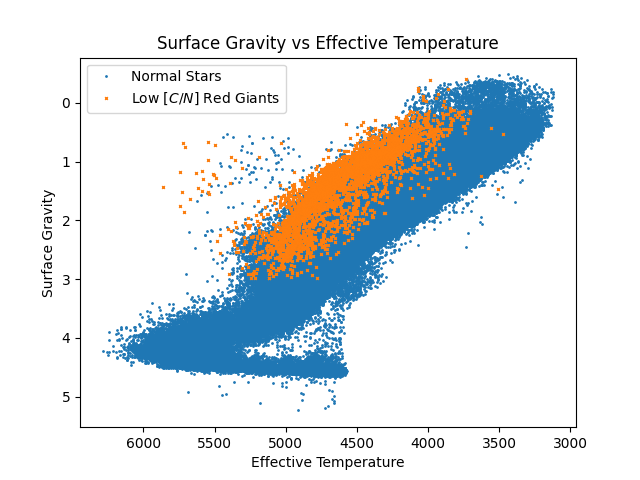
\includegraphics[width=\columnwidth/3]{Figures/AGBProof.png}
    \caption{Verifying whether low \CN stars are AGB stars. Orange data points are for low \CN red giants while the blue data points consist of all the stars in the APOGEE data set. The orange spots that are above the main group of stars are potential AGB stars.}
    \label{fig:AGB_PROOF}
\end{figure}

FYI: the label command can be used just to mark some arbitrary place (e.g. you can label a section or a paragraph if you want to cite them later).
\end{frame}

\begin{frame}[fragile]

Structure of a figure
\begin{verbatim}
\begin{figure}
    \centering
    \includegraphics[additional commands]{location of figure}
    \caption{random text}
    \label{label can be used to reference image}
\end{figure}
\end{verbatim}

The figure on the previous slide uses:

\begin{verbatim}
\begin{figure}
    \centering
    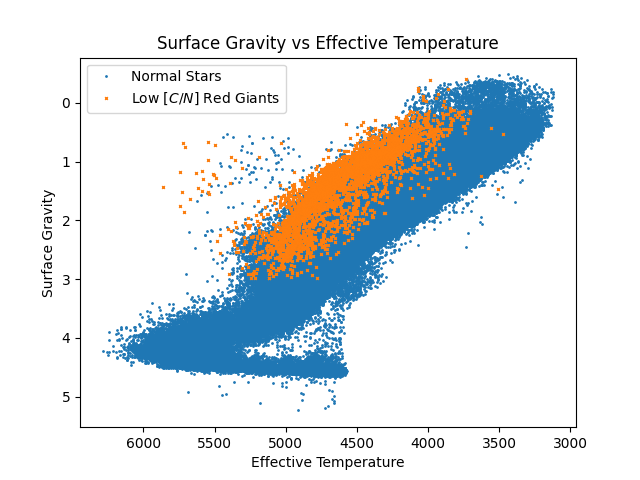
\includegraphics[width=\columnwidth/3]{Figures/AGBProof.png}
    \caption{Verifying whether low \CN stars are AGB stars...}
    \label{fig:AGB_PROOF}
\end{figure}
\end{verbatim}

We can reference the figure \ref{fig:AGB_PROOF} now that its labeled using:
\begin{verbatim}
    \ref{fig:AGB_PROOF}
\end{verbatim}

    
\end{frame}

\begin{frame}

Task:
\begin{itemize}
    \item Include JWST image 
    \begin{itemize}
        \item Make sure it fits
        \item Include a caption
        \item Label it something sensible and reference it
    \end{itemize}
\end{itemize}
    
\end{frame}

\begin{frame}[fragile]
Solution:
\begin{verbatim}
\begin{figure}
    \centering
    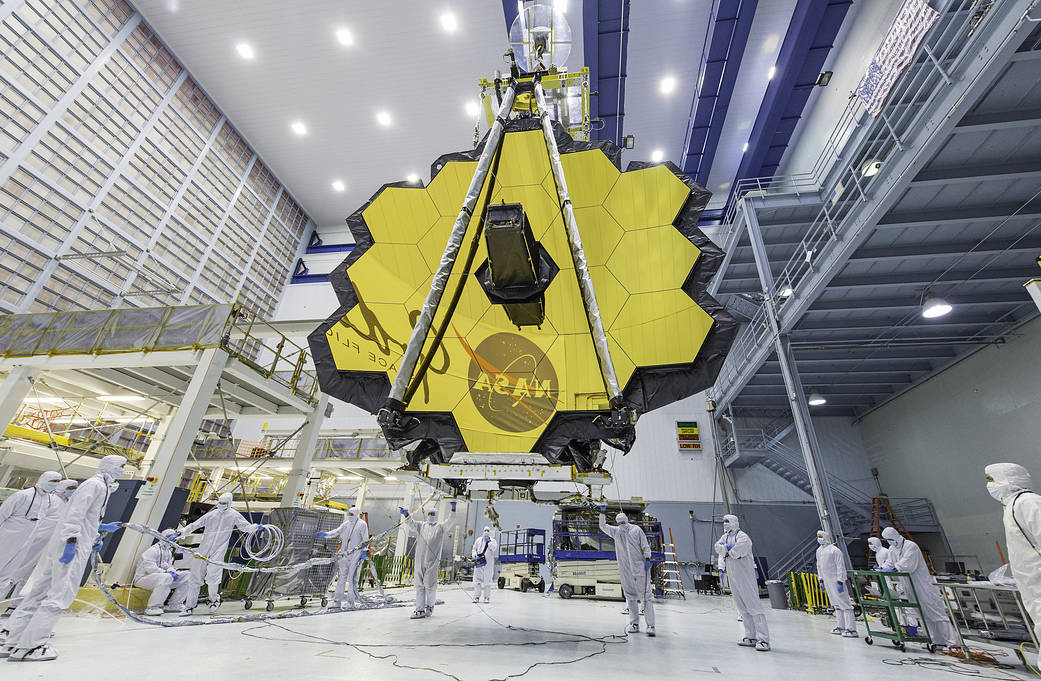
\includegraphics[width=\columnwidth]{photos/jwst.jpg}
    \caption{coolio spaghettio}
    \label{jswt}
\end{figure}

Figure \ref{jswt}
\end{verbatim}

\end{frame}

\subsection{Bibliograph}

\begin{frame}[fragile]
In your research folder, there should be a .bib files where you put your bibliography.
\begin{itemize}
    \item When you cite any of the articles in your .bib file, it should automatically be included in your citations at the bottom of your document
    \item To cite any article, simply write (there should be some citations you can use in the template)
    \begin{verbatim}
        \cite{citation}
        \cite{Martell02}
    \end{verbatim}
\end{itemize}

\end{frame}


\begin{frame}[fragile]
To add another citation, simply export citation from your source of choice and add to the .bib file. \\
Make sure that it is in the form BibTeX. \\
It should look something like this (
P.S. you can change the 2023MNRAS.523LL..80B part (this is an alias, so we can change it to make it easier to recognise, e.g. Kirsten23)
P.S.S your articles maybe different as there are many more fields
\begin{verbatim}
    @ARTICLE{2023MNRAS.523L..80B,
       author = {{Banks}, Kirsten A. and {Ho}, ...}
        title = "{CN and CO features: ...}",
      journal = {\mnras},
     keywords = {asteroseismology, stars: evolution, ...},
     ...
}
\end{verbatim}
\end{frame}


\begin{frame}[fragile]
Task:
\begin{itemize}
    \item Find a new citation of ADS and add it to your document
    \item Cite it and find it in your bottom of your compiled PDF
\end{itemize}
\end{frame}


% % Remember to input this to the presentative tex file before compiling.
\section{Results and Discussion}
\subsection{Results}
\begin{frame}
\begin{columns}
   
\begin{column}{0.7\textwidth}
    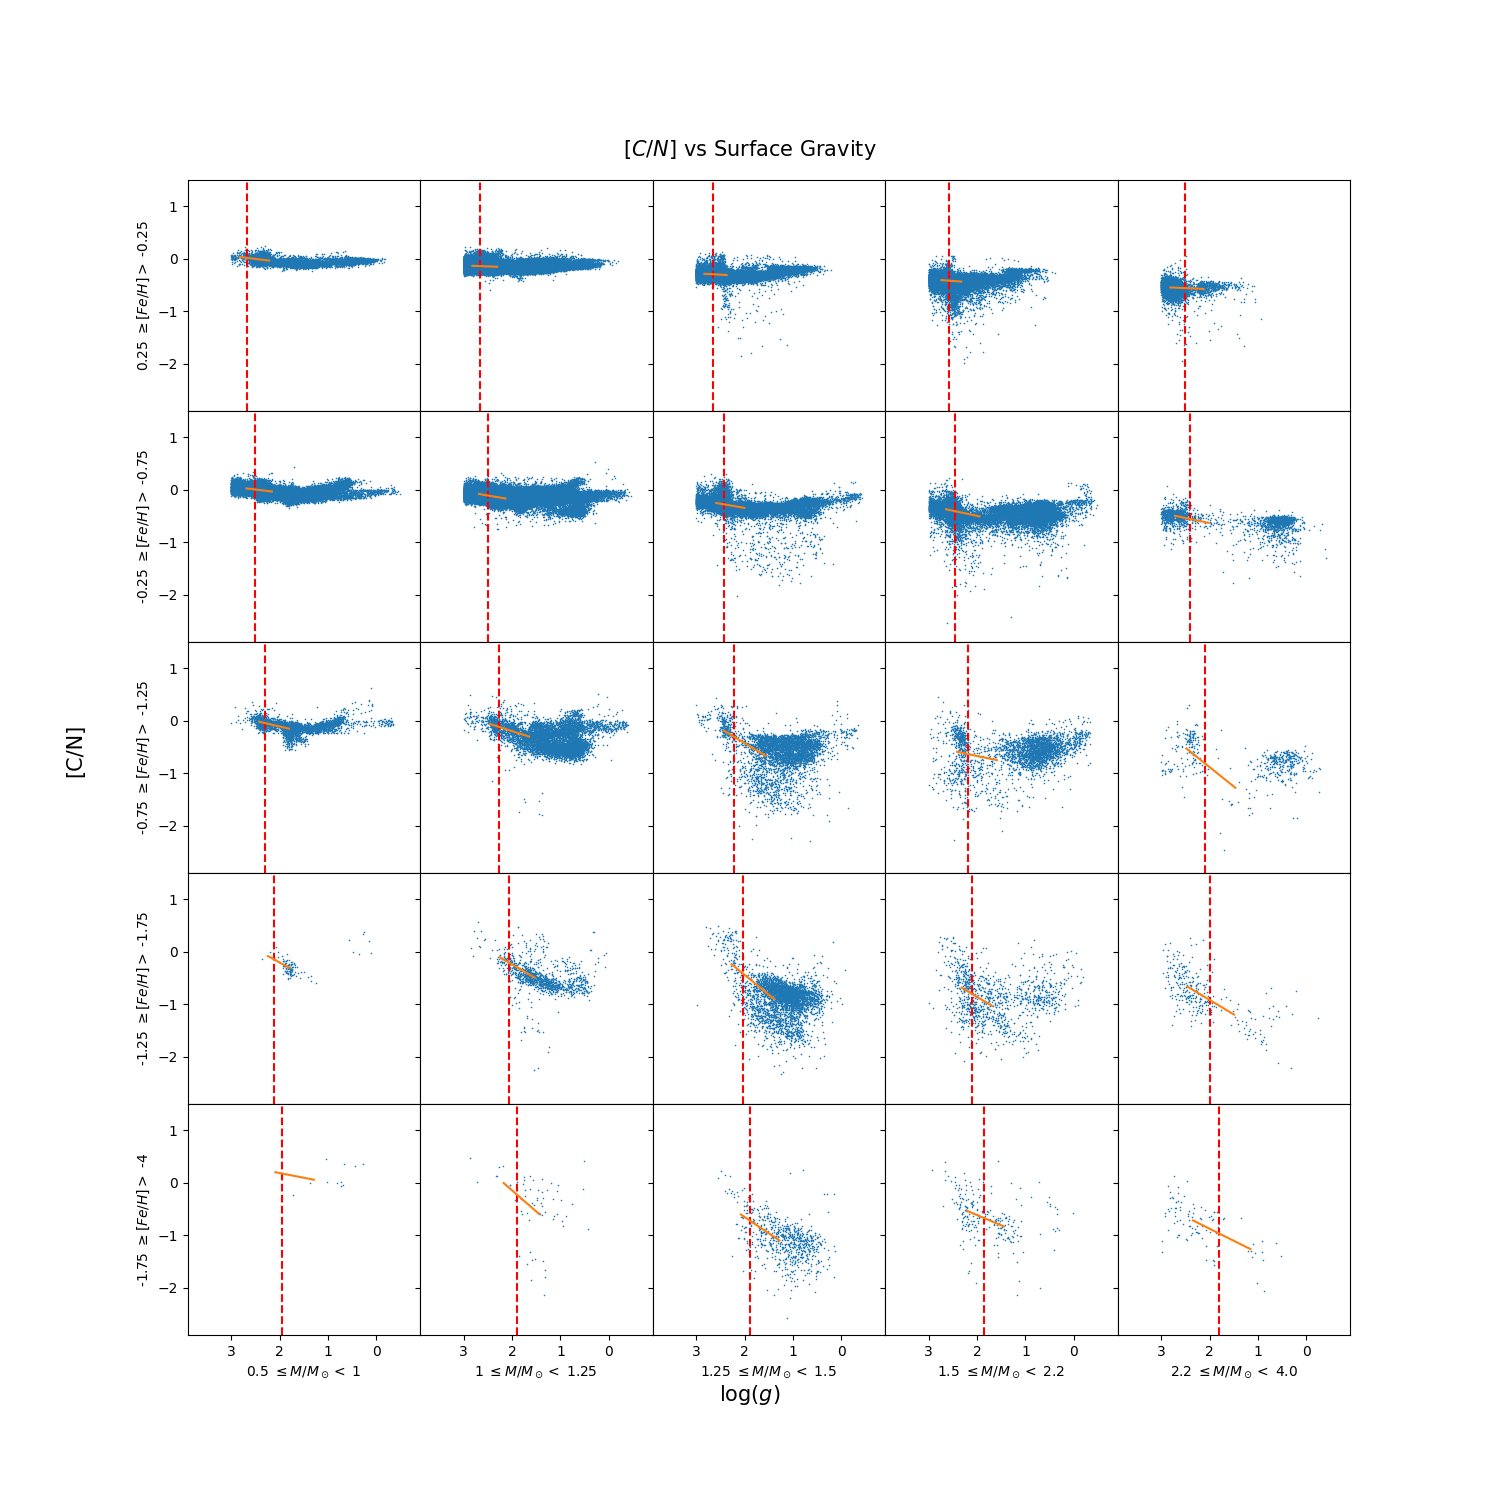
\includegraphics[width=.8\columnwidth]{Figures/DeepMixing.png}
\end{column}

\begin{column}{0.3\textwidth}
    The $\Big[\frac{C}{N}\Big]$ for stars, separated based on mass and metallicity. The vertical red line indicates where deep mixing theoretically begins. The orange lines show the change between average $\Big[\frac{C}{N}\Big]$ before and after deep mixing has theoretically begun
\end{column}
\end{columns}

\end{frame}
\subsection{Discussion}
\begin{frame}
\begin{columns}
   \begin{column}{0.5\textwidth}
        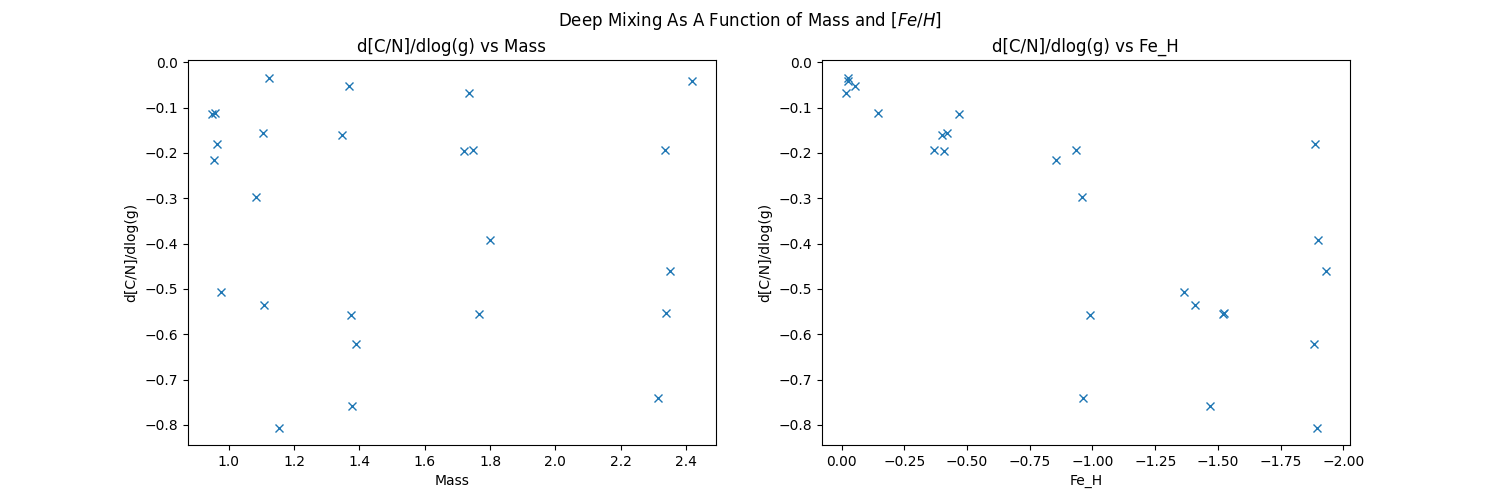
\includegraphics[width=1.2\columnwidth]{Figures/DeepMixingRate.png}
   \end{column}
\begin{column}{0.5\textwidth}
     
   \begin{itemize}
        \item As metallicity decreases, mixing rate increases (EXPECTED)
        \item As mass decreases, mixing rate does not increase (UNEXPECTED)
        \item Mixing occurs for stars with $M>2.2M_\odot$ (UNEXPECTED)
        \item Recovery in \CN for some stars (UNEXPECTED)
        \item Low \CN stars (UNEXPECTED)
   \end{itemize}
\end{column}
\end{columns}
\end{frame}


\begin{frame}
\begin{columns}
   \begin{column}{0.5\textwidth}
        \centering
        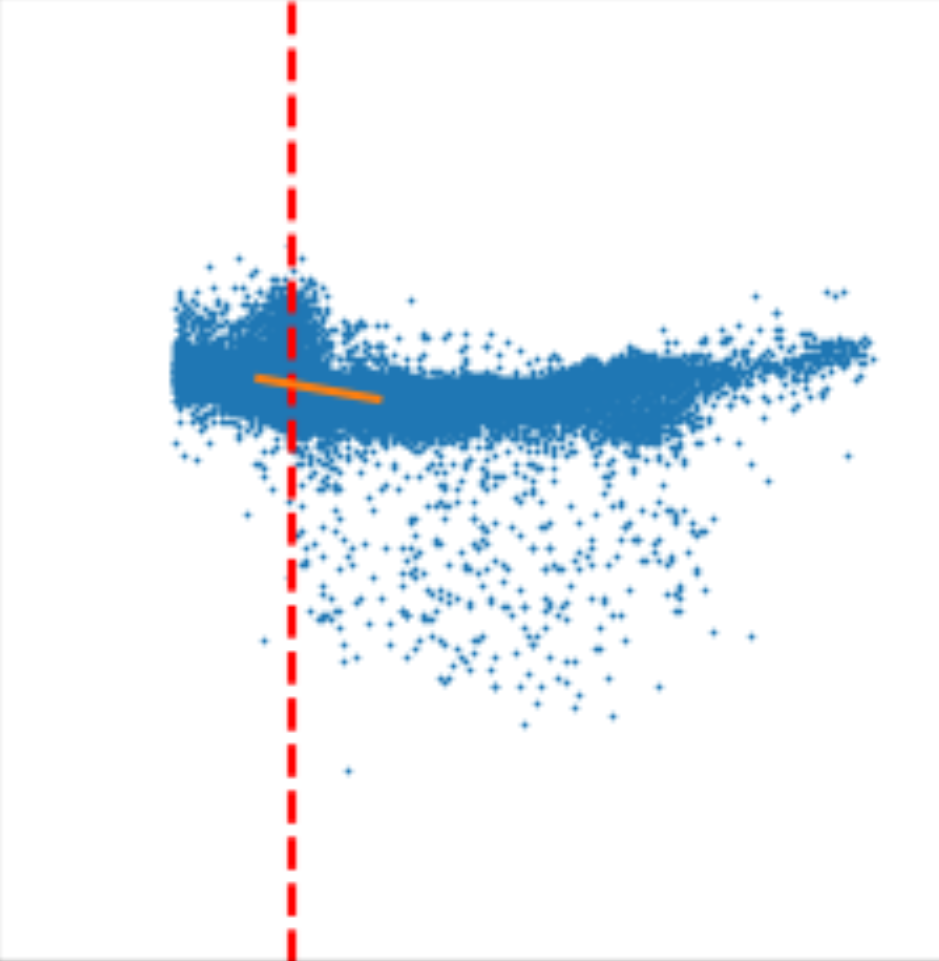
\includegraphics[width=.7\columnwidth]{Figures/Fe(-0.25,-0.75)Mass(1.25,1.5).png}
   \end{column}
\begin{column}{0.5\textwidth}
    The figure shows stars with \abundance{Fe}{H} between -0.25 and -0.75 and mass between 1.25\SM and 1.5\SM.
    \begin{itemize}
        \item We notice that towards the end of the graph (as $\log(g)$ decreases), the \CN has an upwards trend. Why?
        \item We can also notice that there are significant number of stars below the main group. Why?
    \end{itemize}
\end{column}
\end{columns}
\end{frame}


\subsubsection{Low \CN Stars}
\begin{frame}{Globular Clusters}
    \begin{columns}
      \begin{column}{0.7\textwidth}
            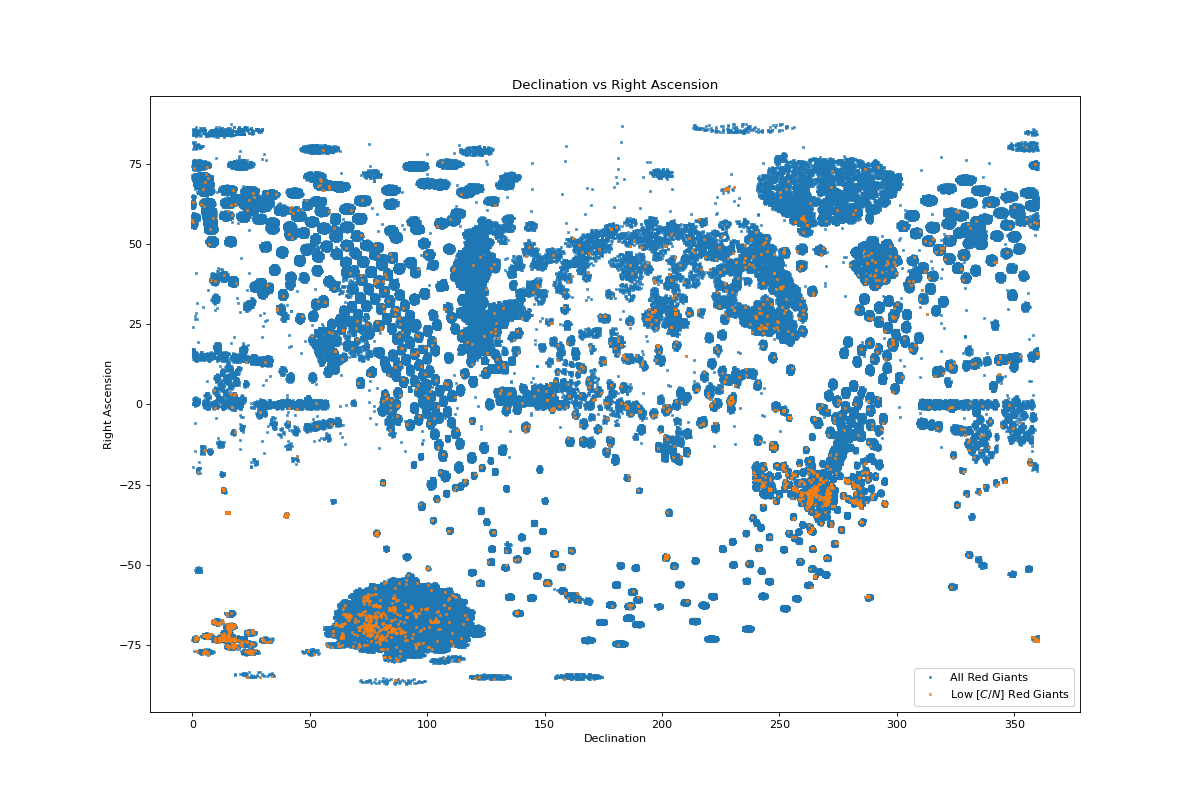
\includegraphics[width=\columnwidth]{Figures/PositionOfLowCNStars.png}
      \end{column}
      \begin{column}{0.4\textwidth}
            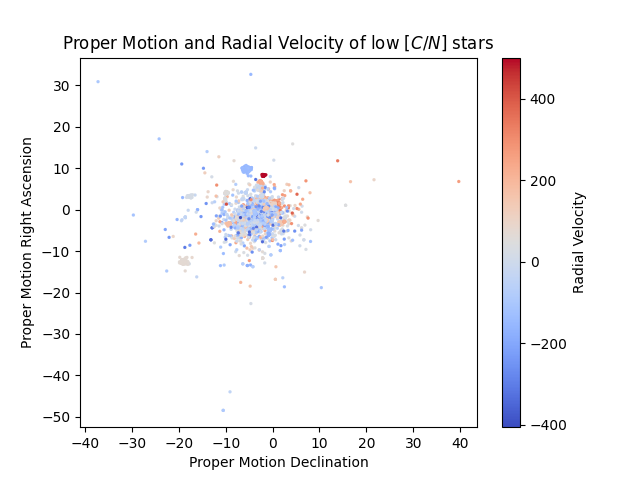
\includegraphics[width=\columnwidth]{Figures/LowCNStarsMotion.png}
      \end{column}
    \end{columns}
    \begin{center}
    Verdict: Globular Clusters do not explain all the low \CN stars.
    \end{center}
\end{frame}

\begin{frame}{Asymptotic Giant Branch (AGB) Stars}
    \begin{figure}
        \centering
        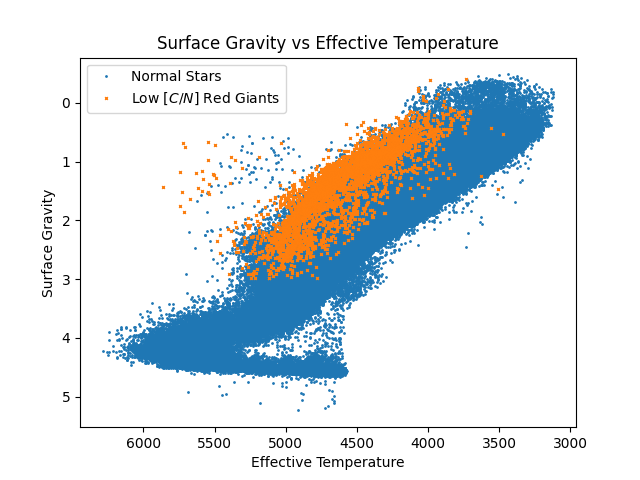
\includegraphics[width=0.5\columnwidth]{Figures/AGBProof.png}
    \end{figure}
    \begin{center}
        Verdict: AGB Stars do not explain all the low \CN stars.
    \end{center}
\end{frame}
\section{Conclusion}

\subsection{Research Paper Structure}
Here is an example of how you can format a research paper
\begin{enumerate}
    \item Abstract
    \item Introduction
    \item Literature Review/Necessary Background Knowledge
    \item Method
    \item Results
    \item Discussion
    \item Conclusion
    \item Ideas for Future Research
\end{enumerate}

\begin{frame}
Research Advice:
\begin{itemize}
    \item Start your report early and do it as you go (keep track of your sources add to your bibliograph periodically)
    \item Schedule time so you can focus on the research (you will most definitely have a few days - few weeks where you have no idea what you are doing) (the hardest part is starting)
\end{itemize}
\end{frame}
\begin{frame}
Task:
\begin{itemize}
    \item Get started with creating a research document
    \begin{itemize}
        \item For those in groups, one person should create a document and share it
        \item Get peoples infos/make a slack group where you can share ideas and plan things out
    \end{itemize}
\end{itemize}
\end{frame}
% \section{Misc}

% This section is a placeholder for you to go over crucial points to takeaway from your presentation.
In summary, during this project, I have:
\begin{itemize}
    \item Crashed my computer 3 times when trying to open up an 18GB file
    \item Written more than 1000 lines of code
    \item 983701 characters in total for meeting minutes and code + other research (if my git command works like I think it does)
\end{itemize}

Also an FYI, we have a lot of spare tongs in the Research Student room on Floor 1 if you would like them owo.
\begin{frame}
\begin{center}
\Huge Thank You!

Special thanks to my supervisor Sarah Martell for having a response time of 2 ms (amongst a ton of other things) 
\end{center}
\end{frame}
% % The appendix tex file gets inputted after the /appendix command in the main tex file.
% Treat your appendices as you would regular chapters, sections and subsections, and they would be automatically discounted as appendices.

\section{Appendix}
\subsection{Appendix I} \label{app1}
\begin{frame}
    \begin{remark}
    This is what an appendix would look like.
    \end{remark}
    \begin{exampleblock}{Example}
    {\gray \lipsum[2][1-20]}
    \end{exampleblock}
\end{frame}

\subsection{Appendix II} \label{app2}
\begin{frame}
    \begin{block}{Relevant Title}
    {\gray \lipsum[2][1]}
    \end{block}
    \begin{exampleblock}{Example of Appendix II}
    {\gray \lipsum[4][1-20]}
    \end{exampleblock}
\end{frame}

% Bibliography/References
% \begin{frame}[allowframebreaks]
% 	\frametitle{References}
% 	\nocite{*}
% 	\printbibliography
% \end{frame}

\end{document}